\documentclass[10pt]{article}
\usepackage[a4paper,margin=1.5cm,top=1.2cm,bottom=1.1cm]{geometry}
\usepackage[T1]{fontenc}
\usepackage{lmodern}
\usepackage{microtype}
\usepackage{booktabs}
\usepackage{array}
\newcolumntype{R}[1]{>{\raggedright\arraybackslash}p{#1}}
\usepackage{enumitem}
\usepackage{titlesec}
\usepackage{tikz}
\usetikzlibrary{arrows.meta,positioning}
\usepackage[hidelinks]{hyperref}

\titleformat{\section}{\normalfont\normalsize\bfseries}{\thesection}{0.6em}{}
\titlespacing*{\section}{0pt}{3pt}{1pt}
\titleformat{\subsection}{\normalfont\normalsize\bfseries}{\thesubsection}{0.6em}{}
\titlespacing*{\subsection}{0pt}{3pt}{1pt}
\setlist{itemsep=1pt,topsep=2pt,parsep=0pt,leftmargin=1.2em}
\setlength{\parindent}{0pt}
\setlength{\parskip}{3pt}
\pagestyle{empty}
\emergencystretch=1em

\newcommand{\cfg}[1]{\texttt{#1}}

\begin{document}

\begin{center}
  {\Large\bfseries VieCut 2.0: A Faster Exact Minimum Cut}\\[3pt]
  {\normalsize Christian Schulz \quad$\cdot$\quad November 17, 2026}
\end{center}

\vspace{-2pt}
\textbf{Goal.} Make VieCut's exact minimum cut faster without changing a single computed cut. The exact algorithm
of~\cite{henzinger2019} is unchanged in what it returns; only its implementation is engineered. Every change was
developed with Agentic Algorithm Engineering (AAE)~\cite{aae}: stated as a hypothesis, implemented, measured on a
fixed benchmark of $53$ instances, and kept only if it was faster and left the minimum cut of every instance
unchanged. The study is described in the AAE paper~\cite{aae}, and every kept change it produced is in this
release, including a later round of single-thread improvements; they are listed in full in the summary on the
second page.

\begin{center}
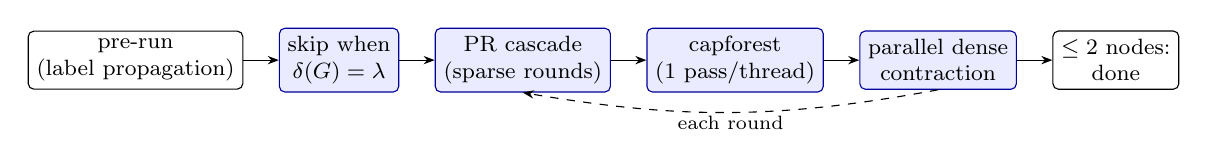
\begin{tikzpicture}[
  box/.style={draw,rounded corners=2pt,align=center,font=\footnotesize,minimum height=7mm,inner sep=3pt},
  new/.style={box,fill=blue!8,draw=blue!60!black},
  >={Stealth[length=4pt]}, node distance=4.5mm]
  \node[box] (lp) {pre-run\\(label propagation)};
  \node[new,right=of lp] (skip) {skip when\\$\delta(G)=\lambda$};
  \node[new,right=of skip] (pr) {PR cascade\\(sparse rounds)};
  \node[new,right=of pr] (cf) {capforest\\(1 pass/thread)};
  \node[new,right=of cf] (con) {parallel dense\\contraction};
  \node[box,right=of con] (done) {$\le 2$ nodes:\\done};
  \draw[->] (lp) -- (skip); \draw[->] (skip) -- (pr); \draw[->] (pr) -- (cf); \draw[->] (cf) -- (con);
  \draw[->] (con) -- (done);
  \draw[->,dashed] (con.south) to[bend left=10] node[below=1pt,font=\scriptsize,inner sep=0pt,fill=white]{each round} (pr.south);
\end{tikzpicture}
\end{center}
\vspace{-6pt}

\section{What changed, and why}
\begin{itemize}
  \item \textbf{The priority queue is sized by the cut, not the graph.} The parallel exact path always built a
  bucket queue with one \cfg{std::deque} per attainable key, sized by the value of the cut --- hundreds of
  gigabytes of empty buckets per round on a large-cut graph, and built once per thread. It now selects between
  that queue, a heap, and an intrusive-list queue by the cut value, as the sequential \cfg{noi\_minimum\_cut}
  already did. This is also why the previous release could not solve $4$ of the $53$ instances at $32$ threads:
  it ran out of memory.
  \item \textbf{The graph is contracted in place, not rebuilt per round}, in both the parallel and the sequential
  loop. On families that contract one vertex per round the old code was quadratic in time and memory; it is now a
  single copy, overwritten each round.
  \item \textbf{A parallel, dense contraction for rounds that collapse the graph.} The sparse contraction
  partitioned by original vertex, forcing a concurrent hash map and a serialized build of the result. A second
  path partitions by contracted vertex, needs neither lock nor hash, and sums parallel edges in a dense array
  that fits in cache when few vertices remain.
  \item \textbf{One capforest pass per thread.} The parallel capforest runs independent traversals, one per
  thread. A feedback rule that reduced the count drove the quantity it measured and collapsed to a single pass;
  it is removed. Whether the passes share their visited array is decided from the graph size before the first
  round.
  \item \textbf{The pre-run's Padberg--Rinaldi reductions are made to cascade} (\cfg{pr\_cascade.h}). The tests
  only fire once contraction has raised the degrees they compare against, so the batch versions, which measure a
  frozen graph, find almost nothing. A cascade contracts on the spot and re-reads degrees, removing whole cycle
  families in a fraction of a second where the capforest needed a round per vertex. It runs on sparse graphs
  only, retires when unproductive, and its merges ride the round's existing contraction.
  \item \textbf{Stamp arrays in the contraction primitives.} \cfg{contractEdge} and \cfg{contractVertexSet}
  found the shared neighbourhood of the two vertices being merged through an \cfg{unordered\_map} rebuilt on every
  merge, on the hottest contraction path. They now use a stamp array (an epoch counter per vertex, so clearing is
  free) that persists with the graph, turning each lookup into an indexed read. On the dense weighted families the
  hash was most of the cost of a round.
  \item \textbf{Smaller edge record, lighter inner loop.} The edge record drops the two fields only the flow
  algorithms read, under \cfg{COMPACT\_EDGES}, for the parallel binaries that cannot reach them. The traversal
  scans the adjacency as one range, uses byte flags, and resolves a vertex's queue position once per update.
  \item \textbf{The pre-run is skipped where the minimum degree already is the cut}, on small sparse graphs,
  where it was pure overhead.
\end{itemize}

\section{Key results}
Geometric mean of the per-instance running time over $53$ instances ($33$ generated families from the 1997
Chekuri--Goldberg--Karger--Levine--Stein study, $20$ real-world $k$-cores of large web and social graphs), on a
$64$-core AMD EPYC.
\begin{center}
\begin{tabular}{@{}lrrr@{}}
\toprule
configuration & before & after & speedup\\
\midrule
exact, $1$ thread   & $25.0$\,s & $2.80$\,s & $8.9\times$\\
exact, $32$ threads & $5.76$\,s & $0.65$\,s & $8.8\times$\\
\bottomrule
\end{tabular}
\end{center}
The $32$-thread ``before'' is the code with every single-thread change applied; the unmodified previous release
cannot solve the whole set at $32$ threads.

\section{New \& compatibility}
\cfg{graph2bin} converts a METIS text graph to a binary form that loads without parsing; \cfg{graph\_io} reads it
transparently. No public interface changed: \cfg{exact}, \cfg{noi}, and the output format are as before, and every
computed cut is identical to the previous release.

\newpage
\section{Summary of changes in this release}
All kept changes from the AAE study~\cite{aae}, grouped by where they apply. A
change marked \emph{parallel} affects only the $32$-thread \cfg{exact} path; one
marked \emph{both} is in the sequential \cfg{noi} loop as well.

\smallskip
\begin{center}
\begin{tabular}{@{}ll R{6.3cm} R{5.5cm}@{}}
\toprule
scope & where & change & effect\\
\midrule
both     & queue        & select heap / deque / intrusive-list by the cut value & solves the $4$ large-cut instances that ran the $32$-thread path out of memory\\
both     & contraction  & contract in place; keep only the graph in use & drops a per-round rebuild that was quadratic on one-vertex-per-round families\\
both     & reductions   & cascading Padberg--Rinaldi (\cfg{pr\_cascade}) on sparse rounds & clears whole cycle families in a fraction of a second where capforest took a round per vertex\\
both     & primitive    & stamp-array shared-neighbourhood lookup in \cfg{contractEdge}, \cfg{contractVertexSet} & removes the per-merge hash map that was most of a round on the dense weighted families\\
both     & traversal    & byte flags; single-probe queue update; scan adjacency as one range; drop dead blacklist & a lighter capforest inner loop on every instance\\
both     & pre-run      & return early when exact; skip when $\delta(G)=\lambda$ on small sparse graphs & removes pure overhead on the easy sparse instances\\
both     & groups       & build only the contraction groups that are read; \cfg{firstContainedVertex} & stops materialising contraction groups nothing reads\\
both     & clustering   & label propagation in vertex order, first-seen tie-break & deterministic clustering; the same cut on every run\\
parallel & contraction  & dense contraction partitioned by contracted vertex (no hash, no lock) & no concurrent map or lock on the rounds that collapse the graph\\
parallel & capforest    & one pass per thread; shared-vs-independent visited by graph size & drops a feedback rule that collapsed the parallel capforest to one pass\\
parallel & batch PR     & parallel Padberg--Rinaldi at the equality boundary & extra reductions once the cut bound is tight\\
parallel & edge record  & \cfg{COMPACT\_EDGES} ($40\!\to\!24$ bytes) for flow-free binaries & a smaller record and a lighter cache footprint\\
build    & flags        & link-time optimisation; \cfg{graph2bin} METIS-to-binary converter & cross-file inlining; binary input that loads without parsing\\
\bottomrule
\end{tabular}
\end{center}

\smallskip
Every change is internal; \cfg{exact}, \cfg{noi}, and the output format are
unchanged, and every computed cut is identical to the previous release.

\begin{thebibliography}{9}
\small
\setlength{\itemsep}{1pt}
\bibitem{aae} D.~A. Bader, A.~Chhabra, E.~Gro{\ss}mann, M.~Henzinger, A.~Noe, and C.~Schulz.
  Agentic algorithm engineering: Improving shared-memory exact minimum cuts.
  Accepted at the 13th DIMACS Implementation Challenge, 2027.
  \href{https://doi.org/10.48550/arXiv.2609.07204}{doi:10.48550/arXiv.2609.07204}.
  Code: \url{https://github.com/CHSZLab/AgenticAlgorithmEngineering}.
\bibitem{henzinger2019} M.~Henzinger, A.~Noe, and C.~Schulz.
  Shared-memory exact minimum cuts.
  In \emph{33rd IEEE International Parallel and Distributed Processing Symposium (IPDPS)}, pages 13--22, 2019.
  \href{https://doi.org/10.1109/IPDPS.2019.00013}{doi:10.1109/IPDPS.2019.00013}.
\end{thebibliography}

\end{document}
